%% Exemplo de utilizacao do estilo de formatacao normas-utf-tex (http://normas-utf-tex.sourceforge.net)
%% Autores: Hugo Vieira Neto (hvieir@utfpr.edu.br)
%%          Diogo Rosa Kuiaski (diogo.kuiaski@gmail.com)
%% Colaboradores:
%%          Cézar M. Vargas Benitez <cesarvargasb@gmail.com>
%%          Marcos Talau <talau@users.sourceforge.net>


\documentclass[openright]{normas-utf-tex} %openright = o capitulo comeca sempre em paginas impares
%\documentclass[oneside]{normas-utf-tex} %oneside = para dissertacoes com numero de paginas menor que 100 (apenas frente da folha) 


\usepackage[alf,abnt-emphasize=bf,bibjustif,recuo=0cm, abnt-etal-cite=2, abnt-etal-list=99]{abntcite} %configuracao correta das referencias bibliograficas.

\usepackage[brazil]{babel} % pacote portugues brasileiro
\usepackage[utf8]{inputenc} % pacote para acentuacao direta
\usepackage{amsmath,amsfonts,amssymb} % pacote matematico
\usepackage{graphicx} % pacote grafico
%\usepackage{times} % fonte times

%--- Este trecho de código arruma as aspas
\usepackage [autostyle, english = american]{csquotes}
\MakeOuterQuote{"}
%---

%--- Este trecho de código arruma a numeração das figuras e tabelas
\usepackage{chngcntr}
\counterwithout{figure}{chapter}
\counterwithout{table}{chapter}
\counterwithout{table}{section}
\counterwithout{table}{subsection}
%---

%Podem utilizar GEOMETRY{...} para realizar pequenos ajustes das margens. Onde, left=esquerda, right=direita, top=superior, bottom=inferior. P.ex.:
%\geometry{left=3.0cm,right=1.5cm,top=4cm,bottom=1cm} 

% ---------- Preambulo ----------
\instituicao{Universidade Tecnol\'ogica Federal do Paran\'a} % nome da instituicao
\programa{Engenharia de Computação} % nome do programa
\area{Engenharia de Computação} % [Engenharia Biom\'edica] ou [Inform\'atica Industrial] ou [Telem\'atica]

\documento{Proposta de Trabalho de Conclusão de Curso} % [Disserta\c{c}\~ao] ou [Tese]
\nivel{Bacharelado} % [Mestrado] ou [Doutorado]
\titulacao{Bacharel} % [Mestre] ou [Doutor]

\titulo{\MakeUppercase{Desenvolvimento de um Sistema de Criptomoeda Centralizado}} % titulo do trabalho em portugues
\title{\MakeUppercase{Development of a Centralized Cryptocurrency System}} % titulo do trabalho em ingles

\autor{Lucas Andrade de Oliveira Reis} % autor do trabalho
\cita{REIS, Lucas Andrade de Oliveira} % sobrenome (maiusculas), nome do autor do trabalho

\palavraschave{Blockchain, Criptomoeda, Banco, Central, Digital, Bitcoin, Centralizada} % palavras-chave do trabalho
\keywords{Blockchain, Cryptocurrency, Central, Bank, Digital, Bitcoin, Centralized} % palavras-chave do trabalho em ingles

%\comentario{\UTFPRdocumentodata\ apresentada ao \UTFPRprogramadata\ da %\ABNTinstituicaodata\ como requisito parcial para obten\c{c}\~ao do grau %de ``\UTFPRtitulacaodata\ em Ci\^encias'' -- \'Area de %Concentra\c{c}\~ao: \UTFPRareadata.}

\comentario{Proposta de Trabalho de Conclusão de Curso apresentada ao curso de Engenharia de Computação da \ABNTinstituicaodata, câmpus Cornélio Procópio, como requisito parcial para a obten\c{c}\~ao do título de Bacharel em Engenharia de Computação.}


\orientador{Prof. Dr. Lucas D. H. Sampaio} % nome do orientador do trabalho
%\orientador[Orientadora:]{Nome da Orientadora} % <- no caso de orientadora, usar esta sintaxe
%\coorientador{Nome do Co-orientador} % nome do co-orientador do trabalho, caso exista
%\coorientador[Co-orientadora:]{Nome da Co-orientadora} % <- no caso de co-orientadora, usar esta sintaxe
%\coorientador[Co-orientadores:]{Nome do Co-orientador} % no caso de 2 co-orientadores, usar esta sintaxe
%\coorientadorb{Nome do Co-orientador 2}	% este comando inclui o nome do 2o co-orientador

\local{Cornélio Procópio} % cidade
\data{\the\year} % ano automatico


%---------- Inicio do Documento ----------
\begin{document}

\capa % geracao automatica da capa
\folhaderosto % geracao automatica da folha de rosto
%\termodeaprovacao % <- ainda a ser implementado corretamente

% dedicatória (opcional)
%\begin{dedicatoria}
%Dedico este trabalho à minha família que, com muito carinho e apoio, mesmo muito %distante, não mediram esforços para que eu chegasse até esta etapa de minha vida.
%\end{dedicatoria}

% agradecimentos (opcional)
%\begin{agradecimentos}
%Agradeço ao Prof. Dr. Lucas Dias Hiera Sampaio pela oportunidade, apoio e %prestatividade na elaboração deste trabalho. Agradeço também a meus pais, Luiz e %Rosemary e meus irmãos, Leonardo e Larissa.

%\end{agradecimentos}

% epigrafe (opcional)
%\begin{epigrafe}
%Texto da ep\'igrafe.
%\end{epigrafe}

%resumo
\begin{resumo}
As criptomoedas e a tecnologia da Blockchain vem conquistando a atenção de investidores e pesquisadores ao longo dos últimos anos. É a primeira vez na história da humanidade que há uma moeda e um sistema de transações em uma só plataforma, resultando em milhares de estudos e novas aplicações desta tecnologia. Este trabalho traz informações sobre o funcionamento da Blockchain e das criptomoedas e propõe a criação de uma nova moeda virtual centralizada, além de apresentar vantagens e implicações de sua implementação.
\end{resumo}

%abstract
\begin{abstract}
Cryptocurrencies and Blockchain technology have been gaining the attention of investors and researchers over the past few years. This is the first time in the history of mankind that there is a currency and a transaction system on the same platform, resulting in various studies and applications of this technology. This work brings information over the operation of Blockchain and cryptocurrencies, purposing the creation of a new centralized digital currency, in addition to presenting advantages and implications of its implementation.
\end{abstract}

% listas (opcionais, mas recomenda-se a partir de 5 elementos)
%\listadefiguras % geracao automatica da lista de figuras
%\listadetabelas % geracao automatica da lista de tabelas
%\listadesiglas % geracao automatica da lista de siglas
%\listadesimbolos % geracao automatica da lista de simbolos

% sumario
\sumario % geracao automatica do sumario


%---------- Inicio do Texto ----------
% recomenda-se a escrita de cada capitulo em um arquivo texto separado (exemplo: intro.tex, fund.tex, exper.tex, concl.tex, etc.) e a posterior inclusao dos mesmos no mestre do documento utilizando o comando \input{}, da seguinte forma:
%\input{intro.tex}
%\input{fund.tex}
%\input{exper.tex}
%\input{concl.tex}


%---------- Primeiro Capitulo ----------
\chapter{Introdução}
\label{chap:intro}

O campo das criptomoedas tem atraído centenas de bilhões de dólares para sua economia \cite{CoinMarketCap2018} e experienciado um rápido aumento em sua popularidade \cite{Judmayer2017}, induzindo um crescente interesse científico em sua tecnologia. 

Neste capítulo serão apresentadas motivações para o desenvolvimento deste trabalho, além de explicitar o objetivo e evidenciar os trabalhos relacionados a esta proposta. 

\section{Motivação}

A mais famosa das criptomoedas é a Bitcoin, a qual pela primeira vez na história trouxe uma moeda virtual e um mecanismo de transferências em um só sistema. Sua capitalização de mercado nos últimos três anos passou de U\$3,4 bilhões para U\$144,9 bilhões (aumento de 4303\%) e o valor por unidade da moeda aumentou de U\$236,15 para U\$8368,83 (aumento de 3543\%) segundo a \citeonline{CoinMarketCap2018}, evidenciando o otimismo e a confiança de seus investidores.

Como destacadas por \citeonline{Mirzayi2017}, apesar de desvantagens como custo operacional elevado, alta volatilidade e uso em cenários criminosos, diversas vantagens podem ser notadas com a utilização de criptomoedas, tais como: segurança nas transações, privacidade financeira, resistência a fraudes, taxa previsível de geração de novas moedas e ausência de gastos como impressão e distribuição de papel-moeda.

Tais pontos fortes são possíveis graças ao caráter seguro e distribuído dos sistemas individuais de cada criptomoeda, que possuem todos seus registros criptografados e guardados em um livro imutável, a Blockchain \cite{Mirzayi2017}. Esses registros são visíveis para todos os nós da rede, que analisam e verificam se as informações nele armazenadas são verdadeiras. Deste modo, a descentralização acaba por garantir a autenticidade dos dados presentes na Blockchain.

Apesar da grande maioria das criptomoedas ser validada de forma descentralizada (com nós da rede espalhados pelo mundo), há ainda a possibilidade dessa rede ser centralizada e continuar sendo distribuída. É o caso de Blockchains utilizadas em indústrias privadas \cite{Li2017}, onde a rede de computadores interna valida os blocos, porém ninguém de fora da empresa tem acesso aos dados e nem é capaz de validar as informações lá armazenadas. 

A Bitcoin se tornou um ícone do liberalismo econômico, como analisado por \citeonline{Santos2016}, por meio da participação dos mineradores e indivíduos que realizam movimentações financeiras virtuais sem a regulação do Estado. Logo, pouco se aplicou o conceito de Blockchain em um cenário centralizado, como uma moeda digital emitida por banco central.

A implementação de uma moeda virtual centralizada, caso implementada para funcionar em um banco central, traz diversas vantagens para uma nação, como a ausência de gastos com emissão de papel-moeda e transparência nas movimentações de capital para todos os cidadãos.

\section{Objetivo}

Acreditando no potencial disruptivo de uma moeda virtual a um baixo custo de manutenção, é proposto neste trabalho a implementação de um sistema de criptomoeda centralizado, podendo ser aplicada em um cenário nacional, sendo assim regulada por um banco central. Por meio de uma interface gráfica, os usuários poderão transferir dinheiro de uma pessoa a outra, tendo os computadores autorizados como validadores das transações do sistema.

\section{Levantamento Bibliográfico}

Ao pesquisar nas bases de dados IEEE e ACM, nota-se que muito pouco foi desenvolvido na área de Blockchain voltada para sistemas centralizados. A imensa maioria desses sistemas foca em centralizar um livro digital em indústrias, garantindo segurança e transparência em suas aplicações.

Para efeitos de comparação, a busca das palavras-chave "central bank cryptocurrency" na plataforma IEE Xplore retorna apenas três resultados, os quais nenhum de fato tratam sobre o desenvolvimento de uma criptomoeda emitida por um banco central. Já na plataforma ACM Digital Library, uma busca avançada pelos artigos os quais o abstract contenha as mesmas palavras-chave ("central bank cryptocurrency") retorna apenas um resultado, o qual também não trata a aplicação desta proposta de trabalho de conclusão de curso.

Apenas um trabalho que compartilha objetivos com este foi encontrado, a Fedcoin, publicada e encontrada fora de bases de dados científicas oficiais. \citeonline{Koning2016} propõe em sua publicação uma moeda estável emitida por uma unidade federativa. O autor também promove análises estruturais pertinentes sobre alguns detalhes de seu funcionamento, tais como até que ponto os cidadãos devem ter acesso a uma moeda não-tangível emitida por banco central, até que ponto a moeda ofereceria anonimato aos usuários, se deveria ou não ter limite de depósito. 

A Fedcoin é apenas um estudo de viabilidade de uma moeda emitida por banco central, onde o autor traz um modelo a ser seguido e algumas diretrizes que a moeda seguiria para garantir sua eficácia. Tal estudo será de grande valor para o desenvolvimento deste trabalho de conclusão de curso, visto que vários pontos estruturais importantes para a construção de uma criptomoeda centralizada em um banco central já foram discutidos pelo autor.


%---------- Segundo Capitulo ----------
\chapter{Fundamentação Teórica}
\label{chap:fund}

Neste capítulo serão evidenciados os fundamentos teóricos necessários para a realização deste trabalho. Seguindo uma ordem lógica, será explicado o funcionamento de uma Blockchain, uma visão geral sobre as criptomoedas e a Bitcoin (incluindo comparações entre alguns algoritmos de consenso), sistemas baseados na tecnologia da Blockchain e aplicações de Blockchain para sistemas centralizados.

\section{Funcionamento da Blockchain}

Segundo Don Tapscott, "a Blockchain é um livro digital incorruptível de transações econômicas que podem ser programados para registrar não apenas transações financeiras, mas virtualmente tudo que possui valor" \cite{Tapscott2016}.

O funcionamento de uma Blockchain foi idealizado por Satoshi Nakamoto, por meio de seu agora famoso artigo \cite{Nakamoto2008}, publicado em 2008. O documento trazia detalhes sobre o funcionamento de um sistema de pagamentos ponto-a-ponto, chamado de Bitcoin (cuja tecnologia por trás de seu mecanismo fora chamada posteriormente de Blockchain).

Uma Blockchain é, como em sua tradução literal, uma cadeia de blocos, onde cada bloco é formado por um conjunto de dados (no caso das criptomoedas, transações) que são armazenados em um livro de registros distribuído. Uma vez registrados em um bloco, os dados se tornam imutáveis, de modo que uma simples alteração invalide todos os blocos subsequentes \cite{Tasatanattakool2018}.

Um bloco genérico é formado por uma lista de hashes de transações independentes. Quando o bloco atinge sua completude, um algoritmo de hashing utiliza então o hash do bloco anterior, mais todos os hashes das transações do bloco corrente para gerar o hash do bloco atual. O próximo bloco, quando gerado, utilizará novamente o hash do bloco anterior a ele para formar seu próprio hash \cite{Nakamoto2008}.

Devido a cadeia de blocos validada pelos hashes, uma simples alteração em um caracter de uma transação de um dos blocos faria com que a hash do bloco em questão mudasse totalmente, invalidando o hash daquele bloco e, por consequência, todos os outros blocos subsequentes \cite{Iansiti2017}.

Uma vez que o bloco esteja completo, inicia-se o processo popularmente conhecido como mineração. Trata-se na verdade, de um algoritmo de prova de trabalho (do inglês, proof-of-work, PoW) no qual os "mineradores" buscam advinhar um elemento do bloco chamado nonce (number used once), que nada mais é que um número aleatório que entra como fator na determinação do hash do bloco \cite{Nakamoto2008}.

Os mineradores trabalham procurando o valor do nonce que faz com que o hash daquele bloco tenha uma característica pré-definida (no caso da rede Bitcoin, os mineradores tentam encontrar um nonce que resulte em um hash de bloco que inicie com $x$ zeros, sendo $x$ chamado de "dificuldade" da mineração) \cite{Vujicic2018}.

Quando o nonce-objetivo é encontrado, toda a rede é avisada e os outros nós verificam se o bloco é realmente válido. Uma vez que o bloco é considerado válido por 51\% da rede, ele é então adicionado à Blockchain e outro bloco se inicia, trazendo a recompensa aos envolvidos na validação dos dados, de acordo com as políticas de consenso do sistema \cite{Judmayer2017}.

Todos esses elementos fazem com que a Blockchain seja um sistema muito seguro por seu caráter distribuído e que seja perfeitamente aplicável a diversos setores da tecnologia.

\section{Criptomoedas}

As criptomoedas são aplicações da Blockchain para sistemas financeiros. São moedas digitais com seus próprios sistemas de transferência e armazenamento, com suas regras regidas por seu código-fonte. São moedas virtuais que podem ser transferidas de pessoa para pessoa sem a regulação de uma entidade central, seguindo as diretrizes P2P.

\subsection{Bitcoin}

A primeira e mais famosa criptomoeda que surgiu foi a Bitcoin, onde sua criação se deu com a publicação do artigo de Satoshi Nakamoto. Ele propôs um sistema com servidor timestamp P2P distribuído, que serve como um gerador da prova computacional da ordem cronológica de transações \cite{Nakamoto2008}. Seu artigo também evidenciava a solução do problema do gasto-duplo (possibilidade de se gastar uma mesma moeda duas vezes), o qual fora resolvido pela implementação do algoritmo de prova de trabalho.

\subsubsection{Funcionamento Geral}

Seguindo os princípios da Blockchain, uma moeda eletrônica é definida como uma cadeia de assinaturas digitais \cite{Vujicic2018}. Cada transação é definida usando o hash digitalmente assinado da transação anterior juntamente com a chave pública do próximo dono. A chave privada é usada para assinar a transação, enquanto a chave pública é usada para verificação da transação, como mostra a Figura \ref{fig:transaction}. A chave pública é mantida em uma carteira, que pode ser implementada em software, hardware ou online. 

\begin{figure}[ht]
\centering
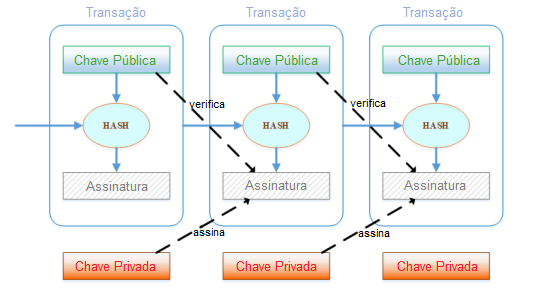
\includegraphics[width=1.0\textwidth]{transaction.PNG}
\caption{Uma transação na rede Bitcoin. Fonte: \citeonline{Vujicic2018}}
\label{fig:transaction}
\end{figure}

O livro de registros do Bitcoin é definido como um sistema de transição de estados, consistindo de um estado que mostra o status de propriedade de todos os Bitcoins e de uma função de transição de estado, sob a forma de transação \cite{Vujicic2018}. A saída dessa função é um novo estado. Os resultados desse processo são mudanças de estado do remetente e destinatário (se o remetente possui Bitcoins suficientes para fazer a transação), ou um erro.

Todas as transações e posses de Bitcoins da rede estão descritas de forma distribuída no livro de registros Bitcoin. Todos os nós da rede P2P detém uma cópia destes registros \cite{Community}. Se um usuário quer enviar uma certa quantidade de moedas para outro, ele pode fazê-lo anunciando publicamente essa transação. Cabe à rede verificar a veracidade desta operação. Contudo, um usuário poderia tentar manipular a rede e emitir mais que uma transação da mesma Bitcoin para usuários diferentes (problema do gasto duplo), o que é impedido pelo mecanismo "proof-of-work".

\subsubsection{Proof-of-Work}

O problema do gasto duplo é previnido na rede Bitcoin por exigir uma prova de trabalho (proof-of-work) de cada nó que verifica uma transação. Os nós tem que fazer cálculos para provar que são membros válidos da rede. Enquanto o poder computacional dos nós honestos for maior que o poder computacional dos atacantes, o sistema continuará consistente e todas as transações legítimas irão ocorrer sem nenhum problema \cite{Tschorsch2016}.

Um conjunto de transações, juntamente com o hash do bloco anterior, mais um nonce, constitui um bloco. Um servidor timestamp faz a hash do bloco e o anuncia publicamente, provando que os dados dentro do bloco tem que ter existido no momento em que o algoritmo de hashing foi executado. O servidor timestamp tem que verificar que o timestamp do bloco é maior que o timestamp do bloco anterior na cadeia e menor que duas horas à frente. Essas hashes são ligadas em cadeia, formando o que é chamado de Blockchain, como na Figura \ref{fig:blockchain}. A grande importância da Blockchain é que todas as transações podem ser consultadas a qualquer momento, sendo publicamente disponível.

\begin{figure}[ht]
\centering
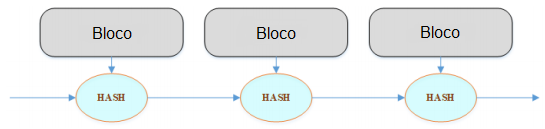
\includegraphics[width=1.0\textwidth]{blockchain.PNG}
\caption{A cadeia de blocos. Fonte: \citeonline{Vujicic2018}}
\label{fig:blockchain}
\end{figure}


O sistema de prova de trabalho que a rede Bitcoin utiliza é similar ao Hashcash \cite{Back2002} e baseado no algoritmo de hashing SHA-256. A prova de trabalho é realizada incrementando o nonce presente no bloco até que o valor do hash produzido seja menor que um número $x$. Uma vez que essa condição é satisfeita, não pode ser desfeita sem repetir os cálculos. 

Na Tabela 1 é exemplificado o papel do nonce em um bloco. Em um cenário de criptomoedas, o texto "Hello world" seria substituído pela lista de transações presentes no bloco. Ainda no exemplo, com o nonce 614 pode ser observado que a saída do hash se inicia com 000, sendo este o chamado hash-alvo (com dificuldade de três zeros) \cite{Drescher2018}.

\begin{table}[ht]
\label{tbl:nonce}
\centering
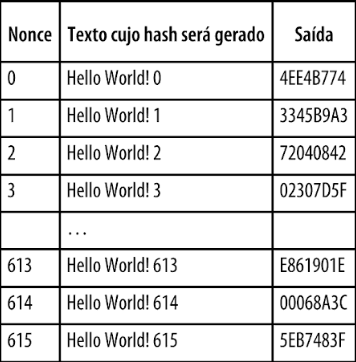
\includegraphics[width=.5\textwidth]{nonce.png}
\caption{Exemplo da relação entre o nonce e o hash. Fonte: \citeonline{Drescher2018}}
\end{table}

Se por algum qualquer dado for modificado por um atacante malicioso, então todos os blocos subsequentes terão hashes inválidos. A regra é que a maior cadeia que possuir a maioria do consenso da rede é a correta. Logo, se um atacante desejar modificar um bloco, ele terá que ter poder computacional para superar a votação da maioria dos nós honestos \cite{Vujicic2018}.

As transações em um bloco passam pelo algoritmo de hash e são estruturadas como uma árvore de Merkle (Merkle Tree). A árvore de Merkle é um tipo de árvore onde a raíz dos nós-folha é uma hash de seus filhos. A Figura \ref{fig:merkle} mostra um bloco que consiste na árvore de Merkle resultante dos hashes das transações. Qualquer inconsistência na árvore será refletida na cadeia. A árvore é utilizada  para liberar espaço de armazenamento ao gravar a Blockchain nos nós. Após as transações serem incorporados em um bloco e esse bloco verificado, a rede descarta todos os hashes da árvore exceto o nó-raíz, incluso no cabeçalho do bloco. Isso ocorre pois a rede Bitcoin implementa uma "verificação de pagamento simplificada" (Simplified Payment Verification, SPV), que não requer que os nós da rede guardem um registro completo das transações, mas só a cópia dos cabeçalhos dos blocos da cadeia mais longa \cite{Nakamoto2008}.

\begin{figure}[ht]
\centering
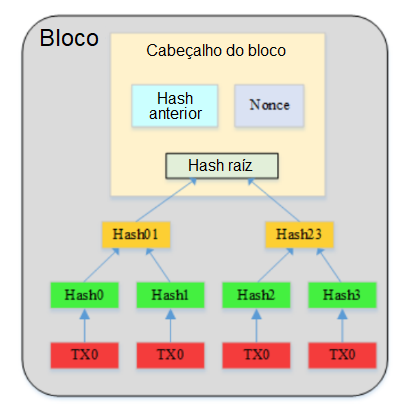
\includegraphics[width=.7\textwidth]{merkle.PNG}
\caption{A árvore de Merkle. Fonte: \citeonline{Vujicic2018}}
\label{fig:merkle}
\end{figure}

A primeira transação em um bloco cria uma nova moeda, que se torna propriedade do criador do bloco \cite{Nakamoto2008}. Essa é a característica que estimula os nós da rede a verificar as transações e permanecerem honestos, além de colocar novas moedas em circulação (já que não existe uma autoridade central emissora de Bitcoins). Essa transação é chamada de "coinbase transaction" \cite{Vujicic2018}. À tarefa de verificar a autenticidade das operações em troca de recompensa, é atribuída o nome de "mineração". 

\subsection{Altcoins}

Após o surgimento e consolidação da Bitcoin, outras criptomeodas surgiram ao longo do tempo, cada uma com seu próprio sistema, políticas e particularidades. Por não serem a principal moeda digital, passaram a fazer parte do grupo das moedas alternativas, as "altcoins".

A Ethereum, por exemplo, é uma altcoin que não tem o mercado financeiro como objetivo principal. Ela é uma plataforma de aplicação descentralizada de "smart contracts" (contratos inteligentes), desenvolvida pelo pesquisador e programador Vitalik Buterin. Ela utiliza computação distribuída baseada em Blockchain que permite o processamento de contratos inteligentes em sua cadeia de blocos \cite{Tasatanattakool2018}.

Na rede Ethereum, o estado é formado por objetos chamados de contas, onde cada transição de estado é uma transferência direta de valor e informação entre as contas \cite{Community}. Sendo assim, além de transferência de valores, as contas podem transferir também posses (como casas ou carros) em forma de código, utilizando estruturas condicionais. 

Um outro exemplo de criptomoeda é a Ripple que, segundo \citeonline{Lewis2014}, é descrita como "um banco medieval digitalizado". É tanto uma moeda digital quanto um protocolo de pagamentos. 

Em um banco medieval, Alex transferiria dinheiro para Beth (em outra localidade) da seguinte forma: Alex deposita o dinheiro em um banco e fala uma senha; a agência de Alex então telefona para a agência de Beth e diz a senha; o agente da agência de Beth então aguarda alguém que diga a senha correta; Beth vai até a agência, diz a senha e recebe o dinheiro. 

Dessa forma, os fundos foram transferidos de forma que a moeda não tenha se movido fisicamente. Pode ser observado também que fez-se necessária a presença de um agente de confiança para que a transação fosse completada.

De forma análoga a esse sistema, no sistema da Ripple, lojas e websites fazem o papel de agentes bancários e a ligação telefônica é substituída por mensagens eletrônicas. Alex realiza login em uma gateway Ripple de sua preferência, deposita dinheiro em sua gateway, instrui a liberar fundos para a gateway de Beth, que coleta os fundos por sua própria gateway (não só dinheiro, mas qualquer bem de valor, no caso da Ripple) \cite{Lewis2014}.

\subsection{Mecanismos de Consenso}

Em um cenário distribuído é extremamente necessária a presença de regras que regem o comportamento da rede e determinam o papel de cada nó. Os participantes acordam quanto à existência, valores e histórico dos estados \cite{Chalaemwongwan2018}. Este acordo mútuo é chamado de mecanismo/algoritmo de consenso. 

Nesta seção serão explicitados os dois principais mecanismos de consenso que podem ser aproveitados para realização deste trabalho, os quais surgiram após problemas encontrados em seu precursor (proof-of-work).

\subsubsection{Problemas com o Proof-of-Work}

Um grande problema de criptomoedas que fazem uso do algoritmo de consenso de prova de trabalho (proof-of-work) é o alto custo operacional para sustentar a rede. De acordo com o site \citeonline{Digiconomist2018}, o gasto de energia elétrica com mineração na rede Bitcoin chega a 65,8TWh, o necessário para fornecer energia para 6 milhões de casas estadunidenses. Isso ocorre pois o algoritmo de prova de trabalho faz com que os mineradores compitam uns contra os outros, resultando em muitos cálculos desnecessários, em troca da recompensa da mineração.

O proof-of-work também acarretou no surgimento das "pools de mineração", uma espécie de rede virtual de computadores que distribui o trabalho entre computadores ao redor do mundo e, quando encontram o nonce do bloco, distribuem a recompensa da mineração entre os computadores da pool. Essa prática acaba levando à centralização da rede \cite{Beikverdi2015}, podendo acarretar no chamado "ataque 51\%" \cite{Tosh2017}.

\subsubsection{Proof-of-Stake}

Para tentar solucionar esses problemas, surgiu o algoritmo de consenso de prova de participação (proof-of-stake, PoS). O sistema usa um processo de eleição onde um nó da rede é escolhido aleatoriamente para validar o bloco seguinte. 

Para se tornar um validador, um nó precisa fazer um depósito de garantia na rede, chamada de  "participação" e, só então, entra o algoritmo de eleição \cite{Tosh2017}. O tamanho da participação determina as chances de um validador ser escolhido para validar o próximo bloco. Em um cenário fictício, Bob faz um depósito de 1000 moedas e Alice faz um depósito de 100 moedas. Com o mecanismo de prova de participação, Bob passa a ter 10 vezes mais chances que Alice de ser escolhido pela rede para validar o bloco corrente.

Quando um bloco é validado, ele é então adicionado à Blockchain e as taxas de transferências cobradas em cada transação são repassadas ao validador do bloco (que fora escolhido pelo algoritmo de eleição), como forma de recompensa pelo esforço computacional. O que impede um validador de aprovar transações inválidas e fraudar a rede, é o depósito feito por ele anteriormente, antes de ser escolhido pelo algoritmo de eleição. Se um validador agir de forma fraudulenta, parte de seu depósito de segurança será confiscado pela rede, de forma que a recompensa pela validação seja menor que o valor perdido no depósito.

Apesar de todas as vantagens que a prova de participação oferece, alguns pontos fracos podem ser observados. Uma das fraquezas do algoritmo é que a validação dos blocos tende a ser centralizada nas mãos dos nós que possuem maior riqueza, podendo gerar um ciclo vicioso, já que os nós com maior posse continuarão aumentando sua riqueza por receberem as recompensas das validações.

Outra desvantagem deste mecanismo é que, mesmo que um validador valide um bloco fraudulento, apenas terá parte de seu depósito tomado pela rede, podendo voltar a ser escolhido para validar outros blocos no futuro. Para tentar driblar essas e outras falhas, um novo algoritmo de consenso foi desenvolvido, o proof-of-authority.

\subsubsection{Proof-of-Authority}

O algoritmo de consenso de prova de autoridade (proof-of-authority, PoA) é uma forma modificada do proof-of-stake, onde ao invés da participação se dar por valor monetário, se dá na verdade pela identidade de um validador. Nesse caso, a identidade significa a correspondência entre a identificação pessoal de um validador na plataforma com os documentos oficiais desta mesma pessoa.

Disponibilizar identidade como participação significa mostrar voluntariamente quem a pessoa é em troca do direito de validar blocos. Isso significa que tanto os benefícios que um participante obtém, quanto  atitudes negativas que ele possa tomar, são públicas.

Para que o conceito funcione da forma correta, três condições devem ser satisfeitas \cite{POANetwork}:
\begin{enumerate}
\item A identidade tem que ser legítima: precisa haver um padrão e um robusto processo de verificação para garantir que os validadores sejam realmente quem eles dizem que são.
\item Elegibilidade para utilizar identidade como participação deve ser difícil de ser obtida: para que o direito de ser um validador se torne merecido, valioso e desagradável de ser perdido.
\item O procedimento para obtenção de autoridade deve ser o mesmo para todos os validadores: para garantir que toda a rede entenda o processo e possa confiar em sua integridade.
\end{enumerate}

Uma grande vantagem do uso do algoritmo de prova de autoridade sobre o algoritmo de prova de trabalho é a inexistência do processo de mineração. Assim como na prova de participação os nós não precisam competir entre si em troca de recompensa, diminuindo drasticamente o custo de energia para manter a rede \cite{Naumoff2017}.

%https://cointelegraph.com/news/why-blockchain-needs-proof-of-authority-instead-of-proof-of-stake

%quadro comparativo
%proof of work, proof of stake, proof of authority

%https://en.wikipedia.org/wiki/Proof-of-authority+
%https://medium.com/poa-network/proof-of-authority-consensus-model-with-identity-at-stake-d5bd15463256

\section{Sistemas baseados em Blockchain}

Aplicações diferentes utilizam a Blockchain de maneiras diferentes, de acordo com a necessidade de cada uma. É dever do projetista escolher o melhor modelo para trabalhar, levando em consideração os algoritmos de consenso existentes, fazendo adaptações e criando novas formas de se implementar uma Blockchain.

Contudo, nem sempre é indicado que uma aplicação seja armazenada em um livro de registros distribuídos e imutável, como mostra o artigo de \citeonline{Lo2017}. O trabalho estuda quando é viável aplicar os conceitos de Blockchain em um sistema ou se um banco de dados convencional já seria suficiente. Utilizando seu estudo e observando o fluxograma da Figura \ref{fig:suitability}, é notável que a proposta deste trabalho de conclusão de curso poderia ser implementada perfeitamente em uma Blockchain.

\begin{figure}[ht]
\centering
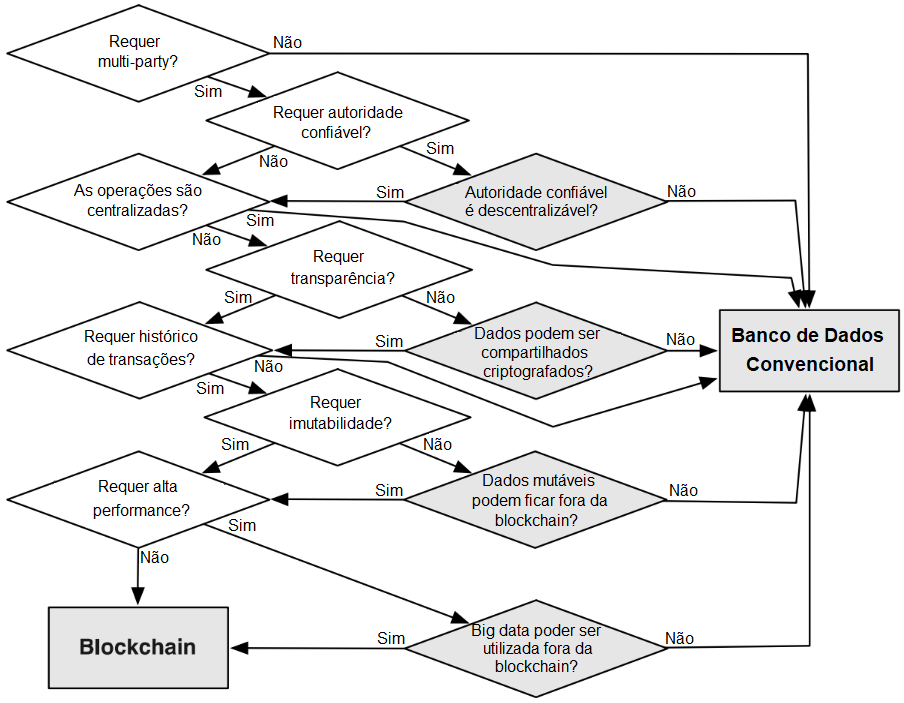
\includegraphics[width=0.9\textwidth]{suitability.PNG}
\caption{Blockchain ou banco de dados convencional? Fonte: \citeonline{Lo2017}}
\label{fig:suitability}
\end{figure}

Como evidenciado por \citeonline{Gatteschi2018}, os princípios da Blockchain podem ser aplicados em diversas áreas para armazenar vários tipos de dados, como transações financeiras, registros públicos, registros privados, identificação, atestados, chaves de bens físicos, bens intangíveis, entre outros.

Uma das aplicações encontradas em pesquisas às bases de dados foi a implementação de um sistema de Autenticação de Arquivos pela Blockchain (Notarizing Files over the Blockchain, NFB). O NFB é um protocolo que garante a comunicação entre uma solução centralizada de arquivamento de documentos e a Blockchain, com o intuito de validar arquivos em uma Blockchain \cite{Magrahi2018}. A tecnologia provê três serviços principais: arquivamento de documentos, recuperação de documentos e prova de existência de documentos. 

Utilizando o protocolo NFB, os usuários podem provar publicamente que um documento existe (ou não), retornando seus metadados indexados na solução de arquivamento seguro e com base nas informações traçadas no Blockchain, durante um período.

Há também uma aplicação que propõe a criação uma plataforma voltada para a indústria de seguros. A ideia por trás do modelo de \citeonline{Raikwar2018} é implementar os processos de uma seguradora em forma de contratos inteligentes (smart contracts), colocando os contratos em uma plataforma distribuída habilitada para Blockchain, tanto para execução dos contratos quanto para armazenamento dos resultados.

Existe também a iniciativa de \citeonline{Koc2018}, que sugere mudanças em sistemas de eleição. Seu trabalho resulta na tecnologia de voto virtual (e-voting), agindo como um contrato inteligente na rede Ethereum, utilizando as carteiras Ethereum e a linguagem Solidity.

Como observado existem várias formas de se utilizar a Blockchain para armazenar informações de forma distribuída e segura, basta o projetista saber a real necessidade de sua utilização e saber aplicar corretamente.


\section{Aplicação de Blockchain em Sistemas Centralizados}

Ao pesquisar nas bases de dados é nítido que a quantidade de estudos a cerca de aplicações de Blockchain em sistemas centralizados é muito menor que a de sistemas descentralizados, o que remete a ideia de que o uso da Blockchain de forma centralizada não foi tão explorada.

A maior recorrência de aplicações centralizadas de Blockchain são provenientes de companhias privadas/indústrias, onde é necessário o armazenamento permanente de determinados registros e, ao mesmo tempo, que haja disponibilidade de infraestrutura para manter o sistema ativo distribuidamente dentro da organização.

O trabalho de \citeonline{Li2017}, por exemplo, propõe uma arquitetura de Blockchain
projetada especificamente para atender os padrões da indústria. A proposta utiliza a ideia de "cadeias de satélites", que podem executar diferentes protocolos de consenso em paralelo, melhorando as premissas de escalabilidade do sistema.

Na mesma proposta é apresentado um modelo interessante, onde os nós da rede podem assumir diferentes papéis: clientes, validadores, auditores ou reguladores. Cada um dos papéis possuindo suas particularidades e finalidades bem definidas \cite{Li2017}.


%---------- Terceiro Capitulo ----------
\chapter{Tecnologias e ferramentas}

Neste capítulo serão tratados alguns detalhes técnicos sobre os processos de desenvolvimento do trabalho proposto.

\section{Implementação}

A implementação será feita dividindo o objetivo em dois problemas distintos: o desenvolvimento do sistema da criptomoeda e a criação da interface gráfica para permitir o registro de transações e visualização das mesmas.

A primeira será desenvolvida em Python, versão 3. A utilização dessa tecnologia se deve à fluência do autor na linguagem e também à existência prévia de bibliotecas que terão papel fundamental no desenvolvimento do sistema (e.g. a pycrypto).

A interface gráfica será desenvolvida para uso desktop, utilizando também a linguagem Python, para integrar o sistema da criptomoeda e permitir a entrada de dados. Como funcionalidade extra, a interface poderá ser transferida para a web, sendo este um objetivo secundário. Caso a implementação do sistema web se concretize, serão utilizadas as tecnologias HTML/CSS, juntamente com Flask, para que possa ser utilizada a linguagem Python no back-end da aplicação.

\section{Processo de desenvolvimento do software}

O desenvolvimento de software se dará utilizando a metodologia Scrum, porém tendo o autor atuando como scrum master e desenvolvedor ao mesmo tempo. 

A escolha deste método de desenvolvimento se dá por se basear em entregas rápidas, contínuas e frequentes, além de ser um método simples e indicado para projetos em que há mudança constante de requisitos. 

%---------- Quarto Capitulo ----------
\chapter{Proposta}

Neste capítulo será explicitada a proposta deste trabalho, tratando aspectos importantes para seu desenvolvimento: objetivos, modelo e cronograma.

\section{Objetivos}

O objetivo principal deste trabalho é desenvolver uma criptomoeda centralizada, que poderá ser aplicada em um cenário privado ou público (com um foco nacional, controlada por banco central), juntamente com uma interface gráfica para entrada de dados no sistema.

Não é um objetivo deste trabalho desenvolver o algoritmo de distribuição (consenso) entre os nós da rede da criptomoeda. Essa decisão foi tomada devido a alta complexidade envolvida em sua implementação e, também, por não ser o foco do trabalho. Todo seu processamento será realizado por uma só máquina.

\section{Modelo}

O sistema da criptomoeda será centralizado em apenas um computador, que realizará a validação dos blocos. Todas as transações poderão ser feitas pelos usuários utilizando um software, que adicionará as transações ao livro de registros da rede (Blockchain), o qual será aberto para consulta.

O sistema será idealizado para ser manutenido pelos funcionários de uma determinada unidade central e tendo como nós da rede os computadores desta determinada entidade, que farão o papel de validadores dos blocos de transações. No caso de uma criptomoeda nacional, os computadores validadores seriam os próprios computadores dos bancos.

No entanto, para efeitos práticos, uma vez que a implementação do algoritmo de distribuição do sistema não é um objetivo deste trabalho, a criptomoeda será validada por apenas um computador central.

\section{Cronograma}

Esta seção traz o cronograma de atividades (dividido em semanas) a serem desenvolvidas para completude do trabalho de conclusão de curso, presente na Tabela 2.

\begin{table}[ht]
\label{tbl:cronograma}
\centering
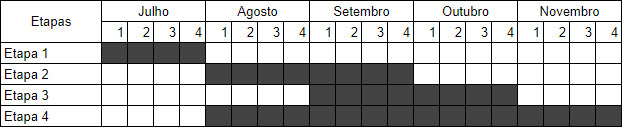
\includegraphics[width=.9\textwidth]{cronograma.PNG}
\caption{Cronograma de desenvolvimento do trabalho. Autoria própria.}
\end{table}
\noindent Etapa 1: Definição do modelo do sistema;\\
Etapa 2: Desenvolvimento do sistema da criptomoeda;\\
Etapa 3: Desenvolvimento da interface gráfica;\\
Etapa 4: Desenvolvimento do trabalho escrito.\\

%---------- Referencias ----------
\bibliography{reflatex} % geracao automatica das referencias a partir do arquivo reflatex.bib


%---------- Apendices (opcionais) ----------
%\apendice
%\chapter{Nome do Ap\^endice}

%Use o comando {\ttfamily \textbackslash apendice} e depois comandos {\ttfamily \textbackslash chapter\{\}}
%para gerar t\'itulos de ap\^en-dices.


% ---------- Anexos (opcionais) ----------
%\anexo
%\chapter{Nome do Anexo}

%Use o comando {\ttfamily \textbackslash anexo} e depois comandos {\ttfamily \textbackslash chapter\{\}}
%para gerar t\'itulos de anexos.


% --------- Lista de siglas --------
%\textbf{* Observa\c{c}\~oes:} a lista de siglas nao realiza a ordenacao das siglas em ordem alfabetica
% Em breve isso sera implementado, enquanto isso:
%\textbf{Sugest\~ao:} crie outro arquivo .tex para siglas e utilize o comando \sigla{sigla}{descri\c{c}\~ao}.
%\sigla{P2P}{Peer-to-peer}
\sigla{PoA}{Proof-of-Authority, prova de autoridade}
\sigla{PoS}{Proof-of-Stake, prova de participação}
\sigla{PoW}{Proof-of-Work, prova de trabalho}

%Para incluir este arquivo no final do arquivo, utilize o comando \input{arquivo.tex}.
%Assim, Todas as siglas serao geradas na ultima pagina. Entao, devera excluir a ultima pagina da versao final do arquivo
% PDF do seu documento.


%-------- Citacoes ---------
% - Utilize o comando \citeonline{...} para citacoes com o seguinte formato: Autor et al. (2011).
% Este tipo de formato eh utilizado no comeco do paragrafo. P.ex.: \citeonline{autor2011}

% - Utilize o comando \cite{...} para citacoeses no meio ou final do paragrafo. P.ex.: \cite{autor2011}



%-------- Titulos com nomes cientificos (titulo, capitulos e secoes) ----------
% Regra para escrita de nomes cientificos:
% Os nomes devem ser escritos em italico, 
%a primeira letra do primeiro nome deve ser em maiusculo e o restante em minusculo (inclusive a primeira letra do segundo nome).
% VEJA os exemplos abaixo.
% 
% 1) voce nao quer que a secao fique com uppercase (caixa alta) automaticamente:
%\section[nouppercase]{\MakeUppercase{Estudo dos efeitos da radiacao ultravioleta C e TFD em celulas de} {\textit{Saccharomyces boulardii}}
%
% 2) por padrao os cases (maiusculas/minuscula) sao ajustados automaticamente, voce nao precisa usar makeuppercase e afins.
% \section{Introducao} % a introducao sera posta no texto como INTRODUCAO, automaticamente, como a norma indica.


\end{document}